\chapter{Materiales y métodos}
\thispagestyle{empty}

\section{Materiales}

En este TFG se generará un conjunto de datos de imágenes sintéticas fotorrealistas a partir de varios modelos 3D seleccionados.

\subsection{Modelos 3D}

Se llevó a cabo un análisis exhaustivo de las bases de datos disponibles de modelos 3D de personas. Tras la búsqueda, se utilizaron diversos conjuntos de datos públicos con el objetivo de crear un conjunto de datos unificado, realista y diverso. En este conjunto, se incluyeron tanto modelos faciales como modelos de cuerpo completo, todos ellos con sus correspondientes texturas.

\subsubsection{Modelos faciales}
Se han seleccionado los siguientes conjuntos de datos: HeadSpace \cite{60}, H3DS-net \cite{61} y DI4D\_UGR\_ANON \footnote{Conjunto de datos proporcionado por el tutor}.

El conjunto de datos de Headspace \cite{60} es un conjunto de imágenes en 3D de la cabeza humana, que consta de 1519 sujetos que llevan gorros de látex ajustados para reducir el efecto de los peinados. Las ventajas de este conjunto son que tienen muy buena resolución y además incluye metadatos útiles para seleccionar un subconjunto de datos adecuado.

\begin{figure}[h]
	\centering
	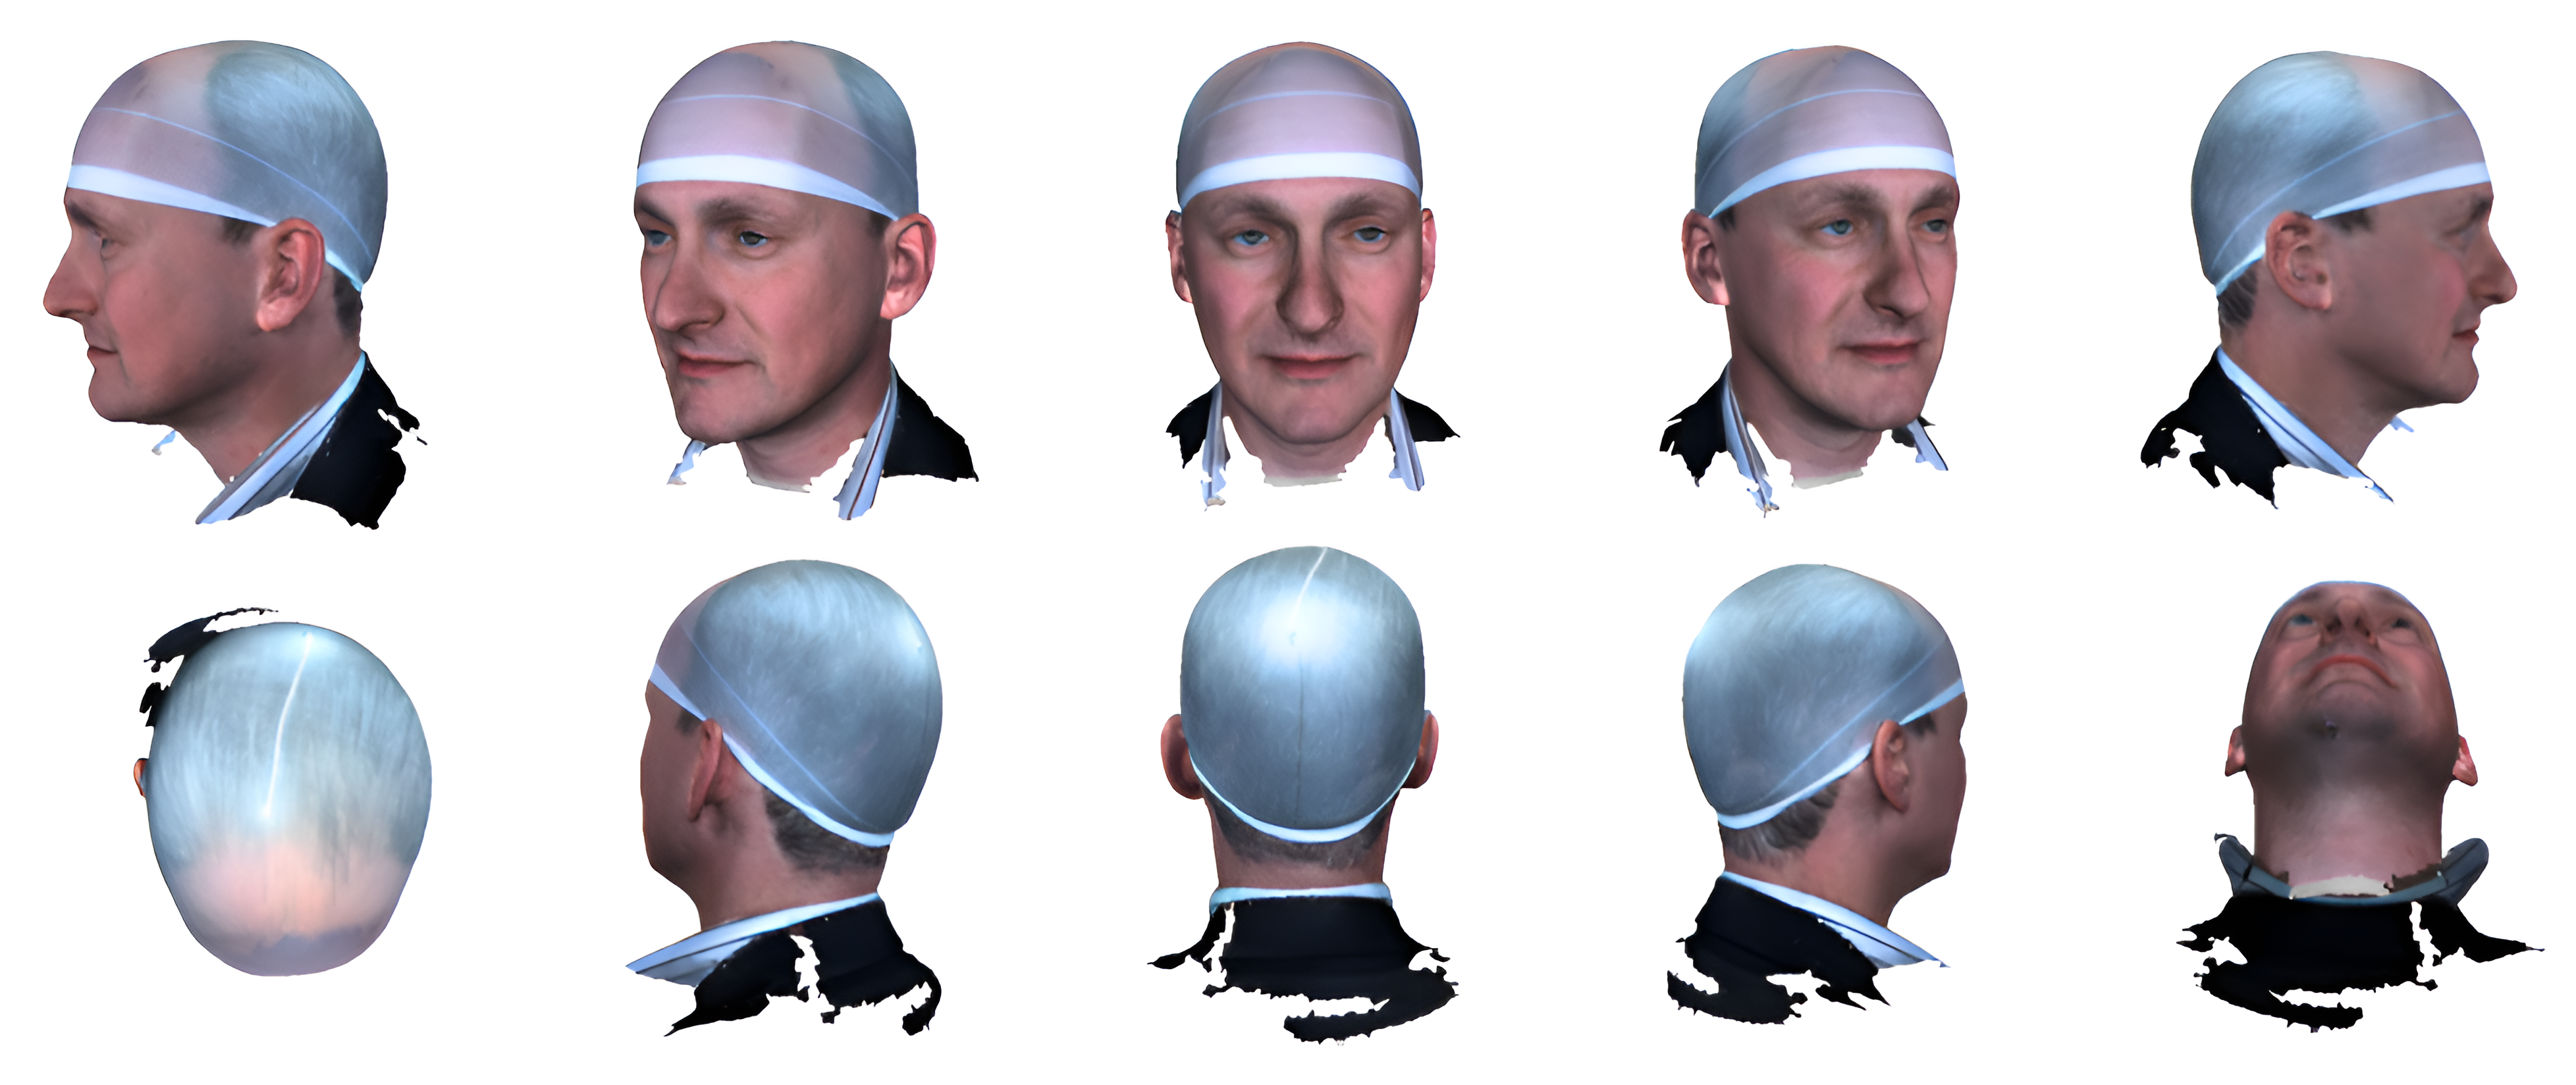
\includegraphics[scale=0.075]{imagenes/cap4/headspace2.png}
	\caption[Ejemplos HeadSpace 3D.]{Ejemplos de modelos en HeadSpace 3D.}
	\label{fig17}
\end{figure}

H3DS-net \cite{61} contiene escaneos texturizados en 3D de la cabeza completa con una alta resolución. Este conjunto comprende un total de 23 modelos, todos ellos con los ojos cerrados, lo que añade una variabilidad adicional.

\begin{figure}[h]
	\centering
	\includegraphics[scale=0.18]{imagenes/cap4/h3dsnet4_1.png}
	\caption[Ejemplos H3DS-net.]{Ejemplos de modelos en H3DS-net.}
	\label{fig18}
\end{figure}

DI4D\_UGR\_ANON es un conjunto de datos creado por la Universidad de Granada...

Si bien se investigaron otros conjuntos de datos como FaceVerse \cite{64} o CASIA \footnote{http://biometrics.idealtest.org/}, estos fueron descartados debido a problemas como la baja calidad, formatos incompatibles y escalas no reales.

\subsubsection{Modelos de cuerpo entero}
Se han seleccionado los siguientes conjuntos de datos: HuMMan \cite{62}, People Snapshot \cite{63} y Render People \footnote{https://renderpeople.com/es/}

HuMMan \cite{62} es un conjunto de datos 3D que consta de 153 sujetos humanos, con una amplia cobertura de sexos biológicos, edades, formas del cuerpo y poblaciones. Cada sujeto contiene 2-3 secuencias, y cada secuencia contiene aproximadamente 20 modelos.

\begin{figure}[h]
	\centering
	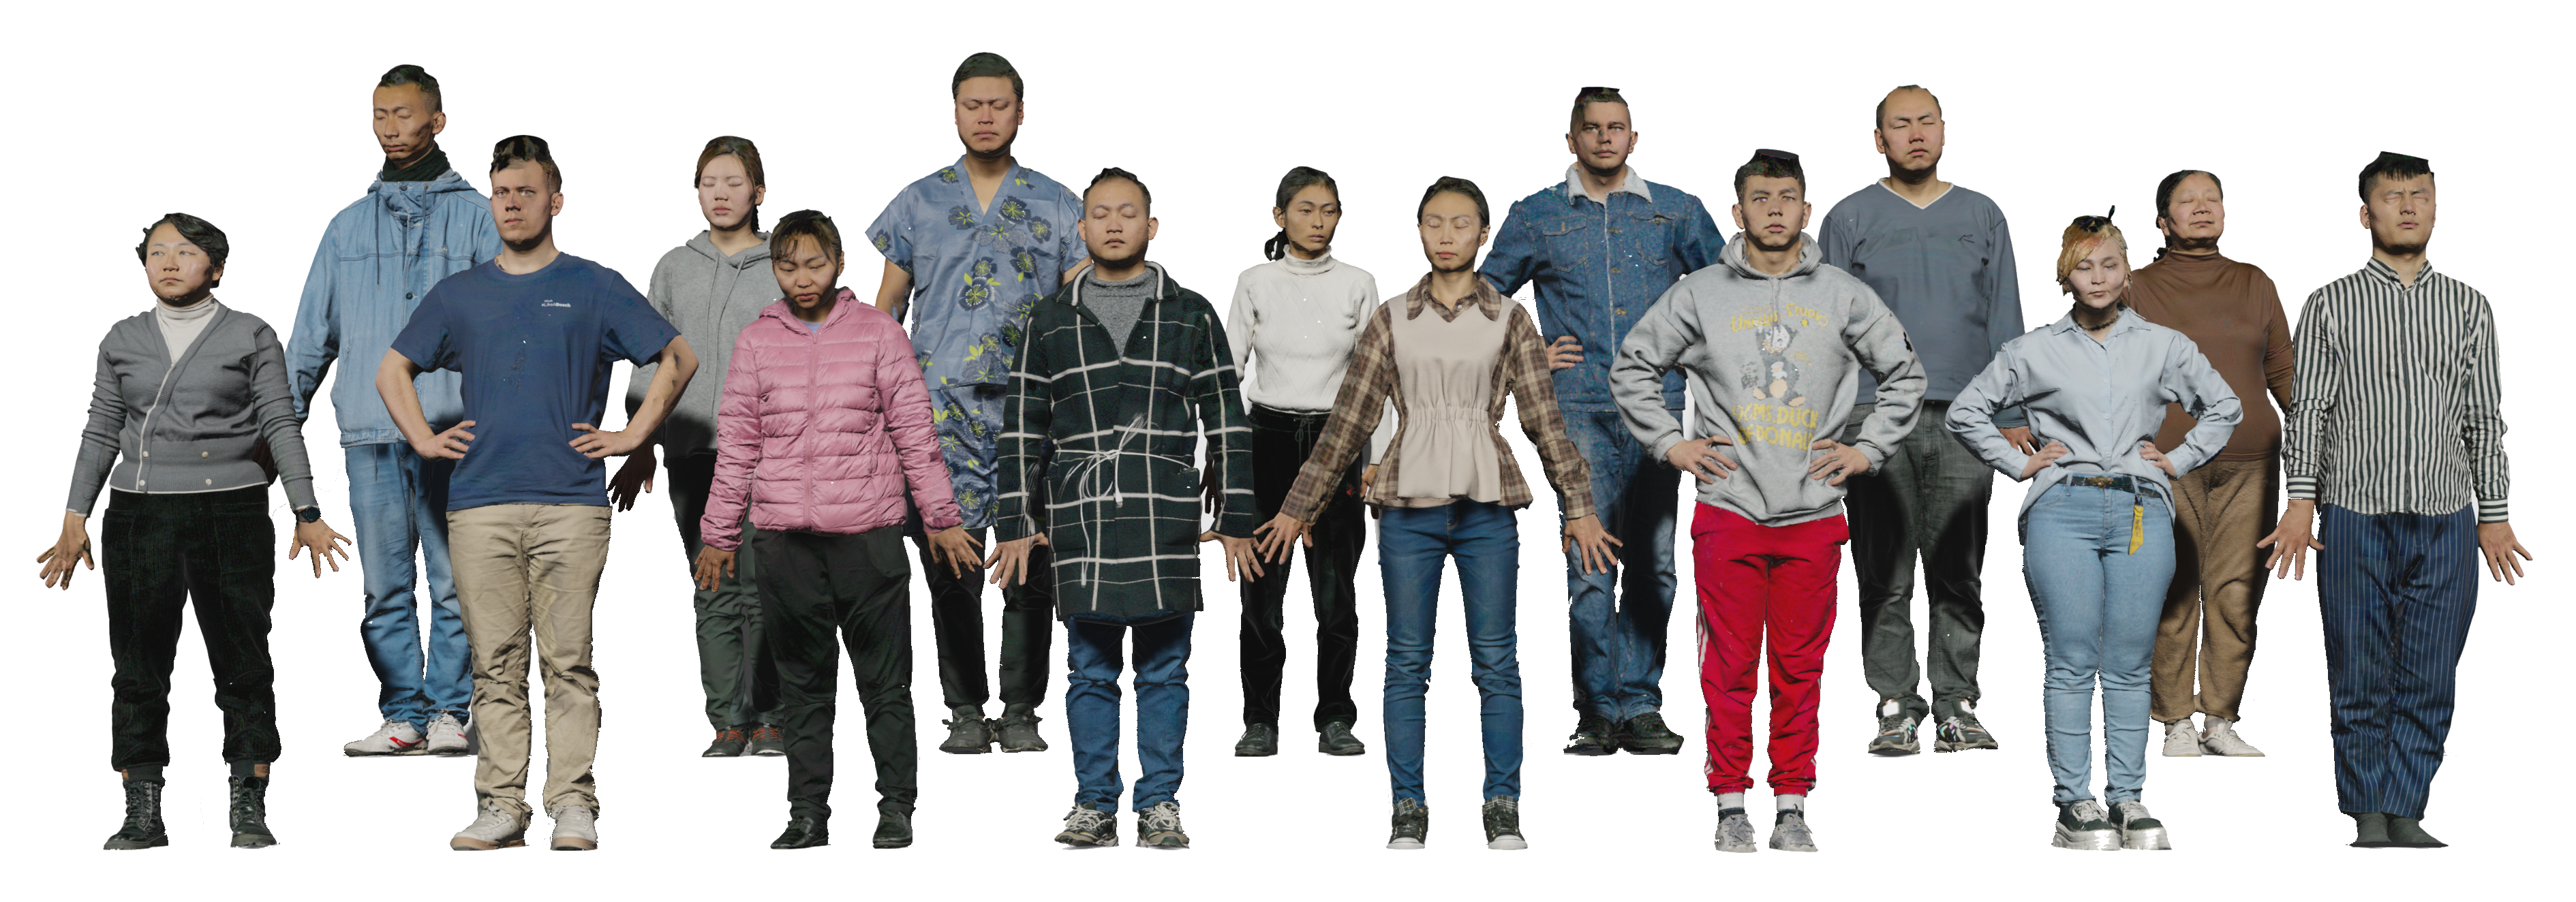
\includegraphics[scale=0.4]{imagenes/cap4/humman2.png}
	\caption[Ejemplos HuMMan.]{Ejemplos de modelos en HuMMan.}
	\label{fig19}
\end{figure}

People Snapshot \cite{63} contiene 24 sujetos 3D en diferentes situaciones tales como casual, deporte y actividades al aire libre.

\begin{figure}[h]
	\centering
	\includegraphics[scale=0.5]{imagenes/cap4/snapshot2.png}
	\caption[Ejemplos People Snapshot]{Ejemplos de modelos en People Snapshot.}
	\label{fig20}
\end{figure}

RenderPeople es una empresa privada especializada en la creación de modelos humanos en 3D. Existen modelos disponibles para comprar, pero dado su costo, hemos decidido emplear exclusivamente aquellos gratuitos que están disponibles. Aunque únicamente hay 2, estos son bastante realistas y presentan situaciones que no se contemplan en los anteriores modelos.

\begin{figure}[h]
	\centering
	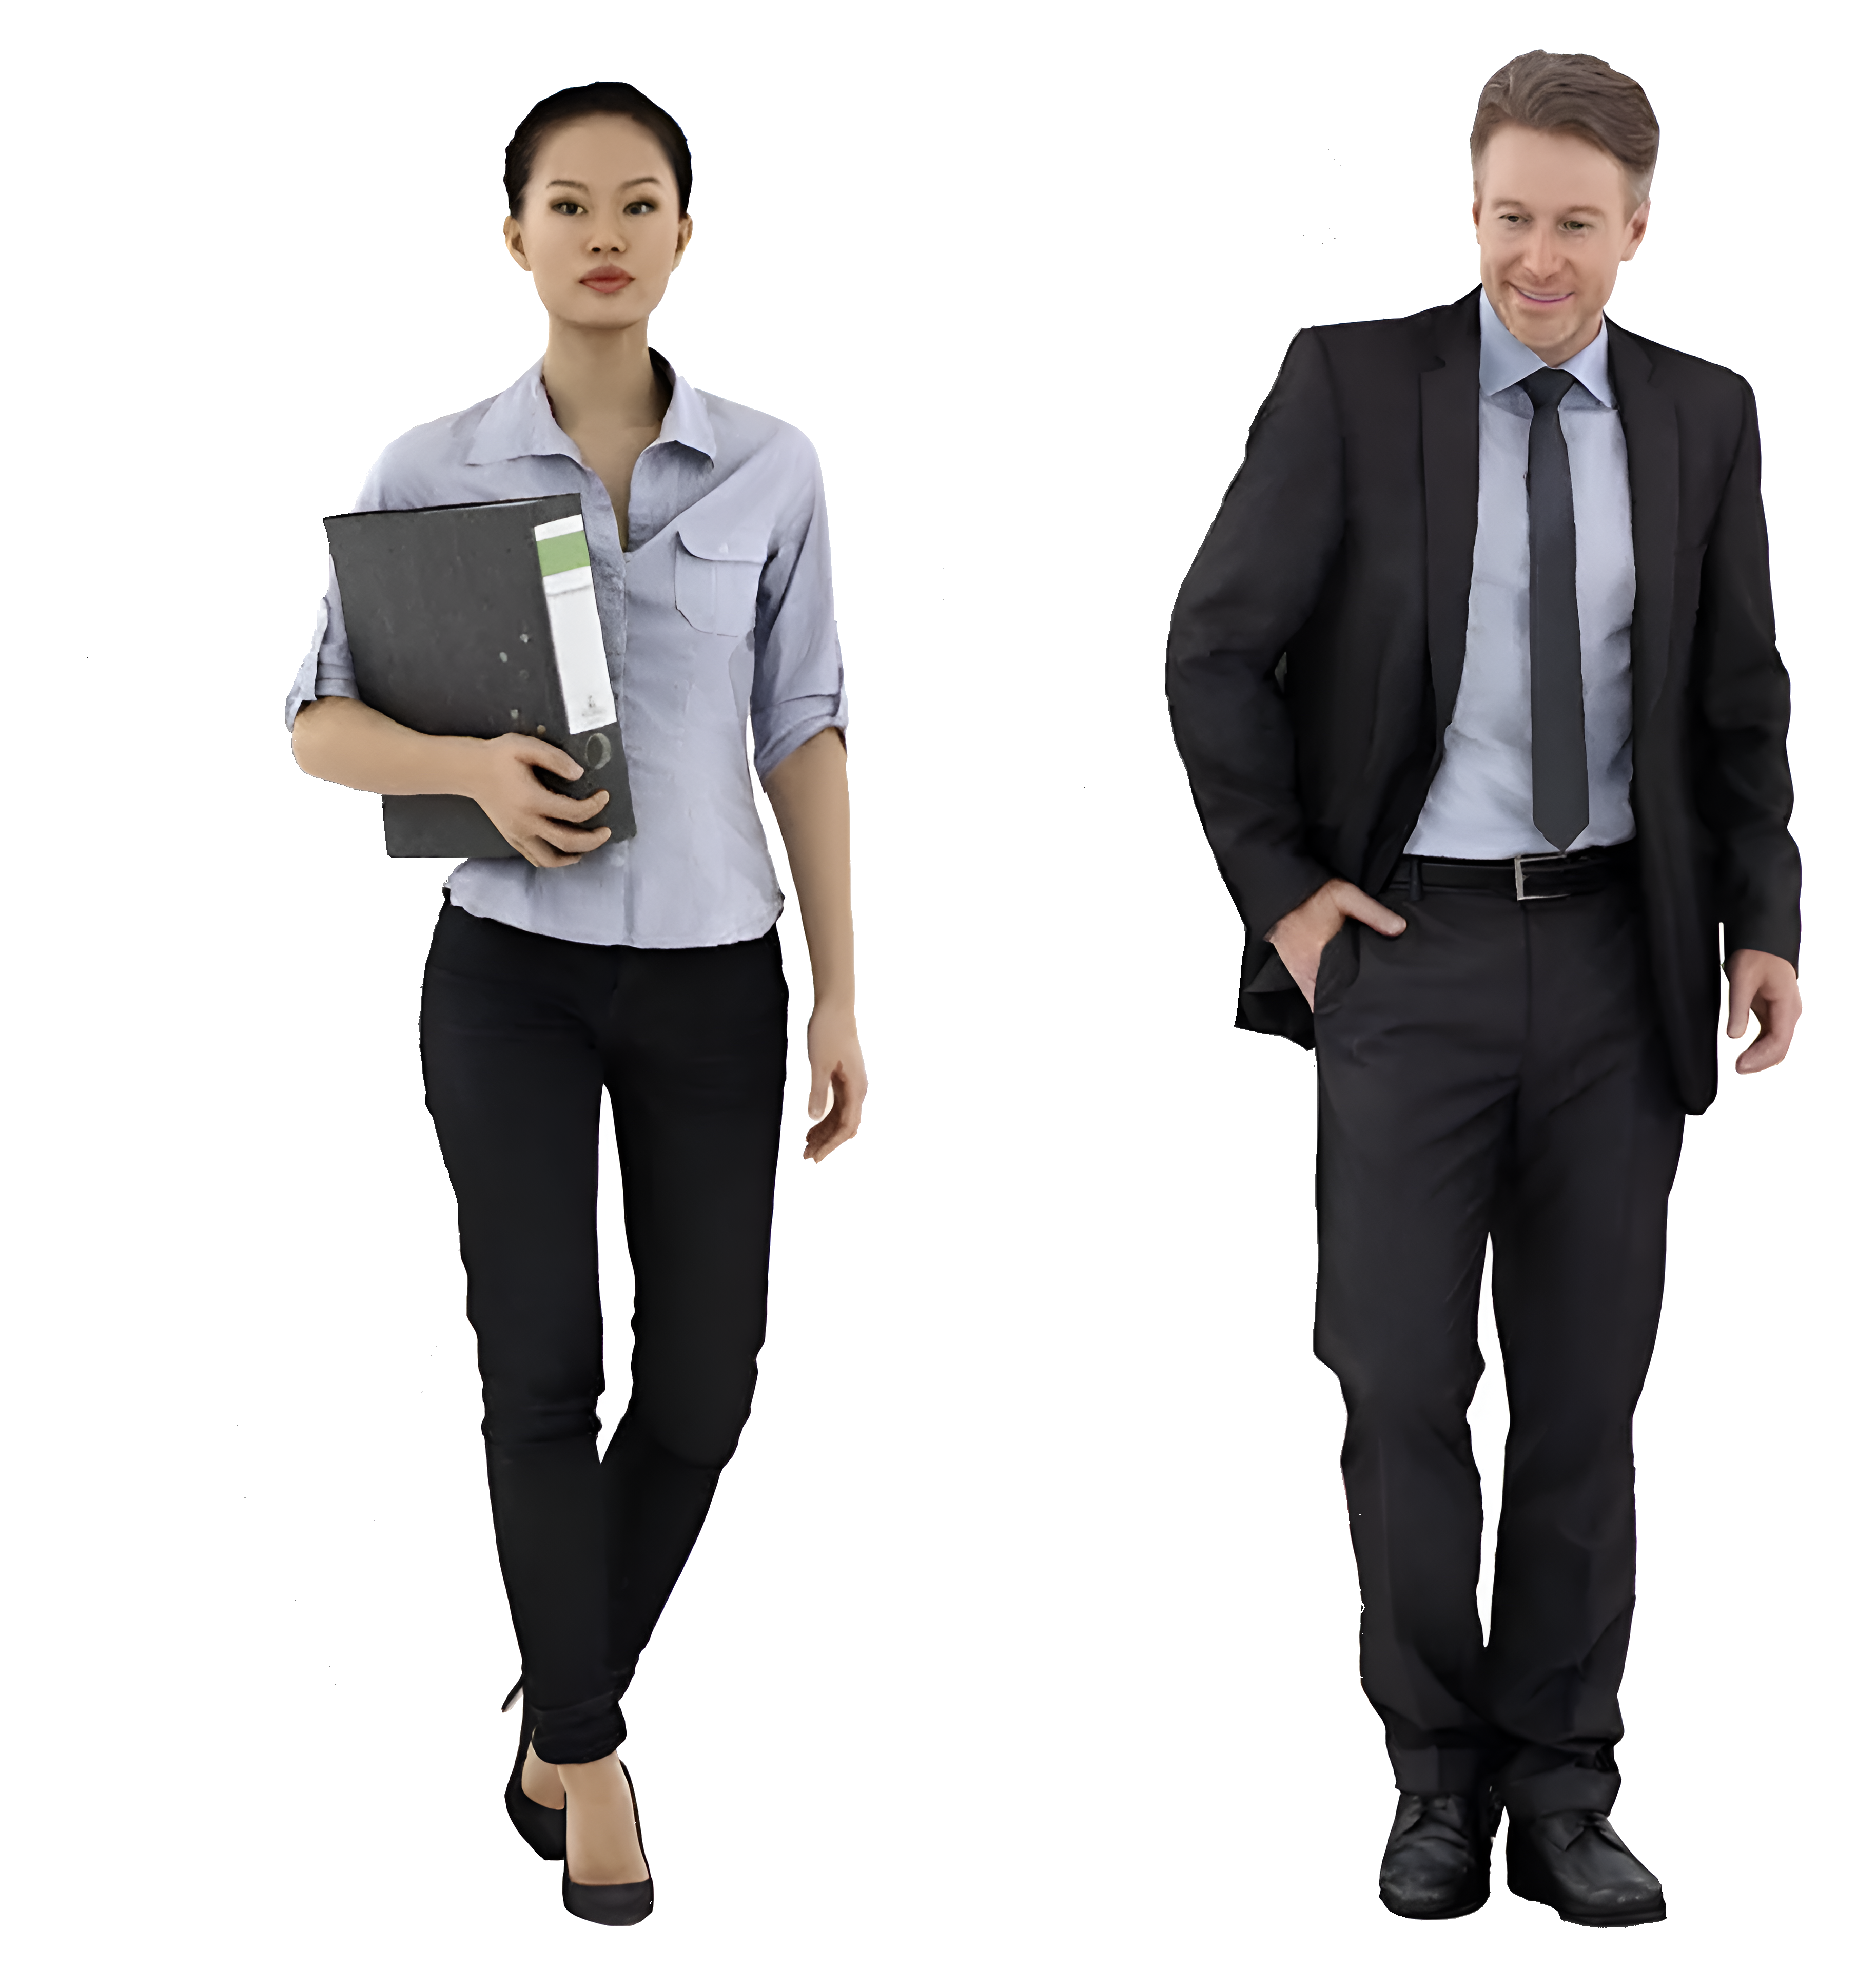
\includegraphics[scale=0.04]{imagenes/cap4/renderpeople2.png}
	\caption[Ejemplos Render People]{Ejemplos de modelos en Render People.}
	\label{fig21}
\end{figure}

\subsubsection{Selección del subconjunto de modelos}

Ante la gran cantidad de modelos disponibles, surge la necesidad de elegir un subconjunto de modelos adecuado, combinando modelos faciales y de cuerpo completo.
En total, se han seleccionado 176 modelos 3D, de los cuales 106 son modelos faciales y 70 son modelos de cuerpo completo.

En primer lugar, de H3DS-net se han seleccionado los 23 modelos, compuestos por 13 masculinos y 10 femeninos, todos ellos de ascendencia europea. 
De HeadSpace, se han elegido 73 modelos, de los cuales 36 son masculinos y 37 femeninos. Esta selección incluye modelos de ascendencia europea, asiática, africana o combinada. Además, todos los modelos son mayores de 14 años.
Respecto a DI4D\_UGR\_ANON, se han seleccionado 10 modelos, compuestos por 6 femeninos y 4 masculinos, todos ellos de ascendencia europea.

Además, se han seleccionado los 2 modelos provenientes de RenderPeople, uno masculino y otro femenino, ambos de ascendencia europea.
De People Snapshot se han seleccionado los 24 modelos, de los cuales 16 son masculinos y 8 femeninos, todos de ascendencia europea.
Finalmente, se han seleccionado 44 modelos de HuMMan, distribuidos en 23 modelos masculinos y 21 modelos femeninos. En este conjunto, 28 modelos son de ascendencia asiática, 11 son de ascendencia africana y 5 son de ascendencia europea.

Estas selecciones se realizaron con el objetivo de incluir la mayor diversidad posible en términos de sexos biológicos y ascendencias, teniendo en cuenta las bases de datos disponibles.

\subsection{Preparación del conjunto de datos}

\subsubsection{Procesamiento de modelos 3D}

Al contar con un conjunto de datos compuesto por múltiples conjuntos, cada uno con una escala específica, ya sea en centímetros o metros, y dispuestos de manera diversa, surge la necesidad de normalizar la escala y alinear los modelos con respecto a un punto de referencia. Para esto, se emplearán los ojos como punto de origen (0, 0, 0), dado que son fácilmente visualizables, se ubican en una posición central y están presentes tanto en los modelos faciales como en los de cuerpo completo. Este procesamiento se produce para luego poder generar correctamente las imágenes a distintas distancias.

La normalización de la escala se lleva a cabo mediante transformaciones de escala, multiplicando o dividiendo por un factor de 100. Esta se realiza solo en algunos modelos, para que todos estén a la misma escala.

Para alinear los modelos, en primer lugar se aplicó un \textit{script} de \textit{Python} para realizar transformaciones (específicas para cada conjunto de datos) con el objetivo de posicionarlos de frente. Posteriormente, se desarrolló un programa en \textit{Python} que utiliza librerías como \textit{VTK}, \textit{PyVista} y \textit{Trimesh} para la manipulación de mallas 3D, junto con \textit{Mediapipe} para la detección de rostros. El proceso implica tener un modelo de referencia ya alineado manualmente, junto con 13 puntos de referencia faciales 3D (incluyendo la nariz, los ojos y la boca) obtenidos mediante \textit{Mediapipe}. Después, dado un nuevo modelo sin alinear, se calculan sus puntos de referencia correspondientes y se determina y aplica la matriz de transformación entre estos puntos y los del modelo de referencia.

A excepción de algunos ajustes manuales en los modelos de HeadSpace y HuMMan, el proceso se automatizó de forma efectiva.

\subsubsection{Generación de imágenes faciales sintéticas}

Una vez procesados los modelos 3D, se procedió a generar el conjunto de imágenes faciales. Para ello, se utilizó un \textit{script} en \textit{Blender} que realiza las siguientes tareas para cada modelo:

\renewcommand{\theenumii}{\arabic{enumii}}

\begin{enumerate}
	\item Carga el modelo y lo posiciona a una distancia específica de la cámara. Se seleccionaron 27 distancias distintas, que van desde 50 cm hasta 6m, con incrementos graduales de 5 cm, 10 cm, 20 cm, 25 cm, 50 cm y 1 m.
	\item Posteriormente, para cada distancia, se ajusta la longitud focal de la cámara. Se utilizaron 4 longitudes focales, incluyendo 27 mm, 35 mm, 53 mm y 83.6 mm.
	\item A continuación, para cada longitud focal, se realizan 14 iteraciones, donde en cada iteración:
	\begin{enumerate}
		\item Se aplica un fondo HDR seleccionado aleatoriamente de un conjunto de 95 fondos HDR descargados de Poly Haven \footnote{https://polyhaven.com}.
		\item Se aplican transformaciones aleatorias de rotación de la cámara con respecto al modelo para añadir variabilidad a las poses. Estas transformaciones incluyen tanto rotaciones horizontales (entre -70º y 70º) para mostrar los modelos desde diferentes perspectivas laterales como se muestra en la Figura \ref{fig22}, así como rotaciones verticales (entre -30º y 30º) para presentar perspectivas más altas o bajas como se muestra en la Figura \ref{fig23}.
		\item Se realizan pequeñas traslaciones de la cámara para evitar que todos los modelos aparezcan centrados en la imagen, añadiendo así una variabilidad extra.
		\item Se ajusta la iluminación y las sombras mediante una lámpara cuya intensidad y posición varían aleatoriamente dentro de unos rango determinados.
		\item Por último, se genera la imagen con un tamaño de 224x224 píxeles.
	\end{enumerate}
\end{enumerate}

\begin{figure}[h]
	\centering
	\includegraphics[scale=0.4]{imagenes/cap4/imagenes_rotacion_vertical.png}
	\caption[Ejemplos de imágenes rotadas verticalmente.]{Imágenes generadas desde perspectivas más altas o más bajas.}
	\label{fig22}
\end{figure}

\begin{figure}[h]
	\centering
	\includegraphics[scale=0.4]{imagenes/cap4/imagenes_rotacion_horizontal.png}
	\caption[Ejemplos de imágenes rotadas horizontalmente.]{Imágenes generadas desde distintas perspectivas laterales.}
	\label{fig23}
\end{figure}

Tras este proceso de generación de imágenes, y considerando que se contaba con 176 modelos 3D, el conjunto total de datos ascendió a 266112 imágenes, es decir, 66528 imágenes por cada longitud focal. Se pueden ver algunos ejemplos de imágenes en la Figura \ref{fig24}.

\begin{figure}[h]
	\centering
	\includegraphics[scale=0.45]{imagenes/cap4/ejemplos_dataset.png}
	\caption[Ejemplos de imágenes generadas para el conjunto de datos.]{Imágenes generadas para el conjunto de datos sintético. Estos ejemplos contienen diferentes sujetos, longitudes focales y distancias.}
	\label{fig24}
\end{figure}

La mejora con respecto al conjunto de datos utilizado en FacialSCDnet \cite{14} es evidente, como se observa claramente en la figura \ref{fig24.1}.

\begin{figure}[h]
	\centering
	\includegraphics[scale=0.3]{imagenes/cap4/figura_FSCDnet.png}
	\caption[Ejemplos de imágenes utilizadas en FacialSCDnet.]{Imágenes utilizadas en FacialSCDnet \cite{14}.}
	\label{fig24.1}
\end{figure}

\section{Métodos}

En este apartado se describen las arquitecturas \textit{deep learning} que se van a utilizar para realizar los experimentos.

\subsection{FacialSCDnet+}

El método FacialSCDnet+, basado en FacialSCDnet \cite{14}, es un enfoque de aprendizaje profundo para estimar la distancia entre el sujeto y la cámara en fotografías faciales. Se basa en una red neuronal convolucional (CNN) diseñada para regresar la distancia métrica de los individuos directamente desde las fotografías faciales. Este método tiene cuatro modelos de aprendizaje, uno por cada longitud focal presente en el conjunto de datos.
A diferencia de FacialSCDnet, este método utiliza un conjunto de datos totalmente sintético, el cual es mucho más realista y diverso. Además, se ha rediseñado el sistema de aumento de imágenes aplicando las operaciones siguientes:

\begin{itemize}
	\item Transformaciones afines: Se aplican rotaciones aleatorias de hasta 15 grados en sentido horario o antihorario, así como traslaciones horizontales y verticales de hasta el 20\% del tamaño de la imagen, con una probabilidad del 100\%. Esta transformación simula diferentes perspectivas de las imágenes.
	\item Emborronado Gaussiano: Se aplica un emborronado gaussiano con un \textit{kernel} de tamaño 5 y un sigma aleatorio entre 0.1 y 2.0, lo que suaviza la imagen, con una probabilidad del 25\%. Esta transformación ayuda a introducir algo de ruido en las imágenes.
	\item Nitidez: Se ajusta la nitidez de la imagen aplicandole un factor de nitidez de valor 2, con una probabilidad del 25\%. Esta transformación simula una mejor definición de las imágenes
	\item Alteraciones de color: Se aplican ajustes aleatorios en el brillo, contraste y tono de la imagen, con un rango de variación entre $\pm$ 0.1 en cada canal, con una probabilidad del 25\%. Esta transformación contribuye a aumentar la diversidad en la apariencia de las imágenes.
	\item Borrado de píxeles: Se borran zonas de píxeles aleatorias de la image. Estas zonas tienen un tamaño de entre el 2\% y el 5\% de la imagen, y la relación de aspecto está entre un 0.5 y un 1.5, dotando a estas zonas de un aspecto más rectangular. Esta transformación tiene una probabilidad del 25\%. Esta transformación introduce un grado adicional de variabilidad y robustez frente a la ocultación parcial de información.
	\item Escala de grises: La imagen se convierte a escala de grises, perdiendo la información de color, con una probabilidad del 25\%. Esta transformación permite al modelo mejorar su invarianza al color.
\end{itemize}

\begin{figure}[h]
	\centering
	\includegraphics[scale=0.4]{imagenes/cap4/augmented_images.png}
	\caption[Transformaciones utilizadas en el aumento de datos.]{Transformaciones aplicadas a las imágenes: a) transformaciones afines, b) emborronado gaussiano, c) nitidez, d) alteraciones de color, e) borrado de píxeles, f) escala de grises.}
	\label{fig25}
\end{figure}

Estas transformaciones aumentan la calidad del conjunto de datos de entrenamiento, mejorando la robustez y la capacidad de generalización del modelo ante diferentes condiciones y variaciones en las imágenes de entrada.

FacialSCDnet+ también utiliza la arquitectura VGG-16 como \textit{backend} para entrenar el modelo de aprendizaje.

\subsubsection{VGG-16}

VGG-16 es una red neuronal convolucional profunda basada en la arquitectura VGGNet \cite{65}. Esta red contiene 16 capas entrenables, como su nombre indica, y destaca por su eficacia en la extracción de características en imágenes.

La red recibe como entrada una imagen RGB de tamaño fijo de 224x224. Esta imagen atraviesa una serie de capas convolucionales, donde se emplean filtros de tamaño 3x3. En estas capas, el \textit{stride} se mantiene constante en 1 píxel y se utiliza un \textit{padding} de 1 píxel para evitar la pérdida de dimensionalidad al aplicar los filtros de convolución 3x3. Cada capa convolucional contiene una capa de activación ReLU detrás.Tras algunas de las capas convolucionales, se realiza un \textit{max pooling} con filtros de 2x2 y \textit{stride} de 2 píxeles, esta operación se realizar para ir reduciendo el tamaño de los mapas de activación. En esta primera parte de la red es donde se extraen las características de la imagen.

Posteriormente, esta primera parte de la red es sucedida por tres capas totalmente conectadas: las dos primeras cuentan con 4096 neuronas cada una, mientras que la tercera realiza la clasificación con 1000 neuronas (una por cada clase). Tras cada una de estas capas, sigue una capa de activación ReLU. La última capa corresponde a la capa de \textit{soft-max} que calcula las probabilidades de pertenecer a cada clase. En esta parte final de la red se realiza la clasificación final de las características extraídas para la tarea de reconocimiento de imágenes.

La arquitectura VGG-16 se puede ver en la Figura \ref{fig26}.

\begin{figure}[h]
	\centering
	\includegraphics[scale=0.1]{imagenes/cap4/vgg-16.png}
	\caption[Arquitectura de la red VGG-16.]{Arquitectura de la red VGG-16. Las dimensiones se muestran en formato: Columnas x Filas x Canales \cite{66}.}
	\label{fig26}
\end{figure}

El uso de convoluciones 3x3 tiene dos ventajas:

\begin{itemize}
	\item Permite aplicar más convoluciones e incrementar la profundidad de la red al tener menos parámetros entrenables.
	\item Combinando las pequeñas convoluciones y la profundidad de la red, se pueden detectar características a pequeña escala, mientras que la agregación de escalas mayores va implícita al pasar de capa.
\end{itemize}

El uso de esta red se justifica por su sencillez y su capacidad para aprender características significativas de las imágenes mediante el bloque de capas convolucionales. 

En FacialSCDnet+, se ha modificado la estructura de la red de manera que se conserva la extracción de características a través de los bloques convolucionales, aprovechando los pesos preentrenados en ImageNet, mientras que en la parte final de la red se incluyen dos capas fully connected con 4096 neuronas cada una, junto con una capa de salida con una sola neurona para abordar el problema de regresión. Se realiza un proceso de fine-tuning, es decir, los pesos de los bloques convolucionales permanecen congelados, mientras que la parte final de la red es entrenada desde cero. En total, la red cuenta con 119,545,857 parámetros para el entrenamiento.

Dado su alto número de parámetros a entrenar, VGG-16 demanda recursos computacionales significativos, sin embargo, su gran rendimiento lo convierte en una opción atractiva para este trabajo.